\documentclass[crop,tikz]{standalone}

\usepackage{amsmath}

\begin{document}

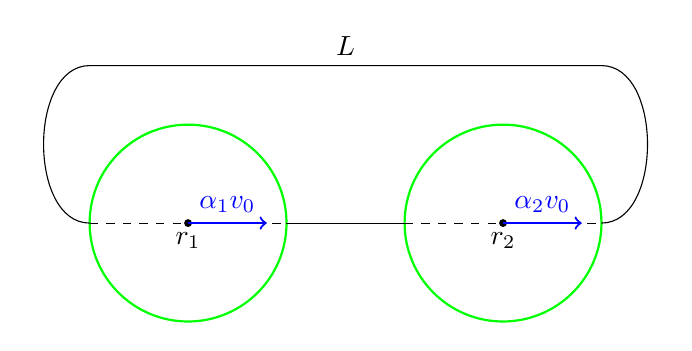
\begin{tikzpicture}
\fill (0, 0) node[below]{$r_1$} circle (0.5mm);
\draw[green, thick] (0, 0) circle (1.25);
\fill (4, 0) node[below]{$r_2$} circle (0.5mm);
\draw[green, thick] (4, 0) circle (1.25);
\draw (1.25, 0) -- (2.75, 0);
\draw (5.25, 0) to[out=0,in=0] (5.25, 2) -- (-1.25, 2) to[out=180,in=180] (-1.25, 0);
\draw (2, 2) node[above]{$L$};
\draw[dashed] (-1.25, 0) -- (1.25, 0);
\draw[dashed] (2.75, 0) -- (5.25, 0);
\draw[thick, blue, ->] (0, 0) -- (1, 0) node[midway, above]{$\alpha_1 v_0$};
\draw[thick, blue, ->] (4, 0) -- (5, 0) node[midway, above]{$\alpha_2 v_0$};
\end{tikzpicture}

\end{document}
